\documentclass[11pt]{article}
\usepackage[utf8]{inputenc}
\usepackage[english]{babel}
\usepackage{bilal2vec}
\usepackage{minted}
\title{CS 486 - Assignment 2}
\author{Bilal Khan\\
\href{mailto:bilal2vec@gmail.com}{bilal2vec@gmail.com}}
\date{\today}

\begin{document}

\maketitle
\tableofcontents

\section{1}

\begin{minted}{text}
  METHOD 1

  node split_order: 1: split on 'christian' feature: 193 i_g = 0.500 n_doc: 1500
    [leaf] pred = 1 n_doc: 35
    node split_order: 2: split on 'atheism' feature: 4662 i_g = 0.500 n_doc: 1465
      [leaf] pred = 1 n_doc: 24
      node split_order: 3: split on 'christians' feature: 1239 i_g = 0.499 n_doc: 1441
        [leaf] pred = 1 n_doc: 19
        node split_order: 4: split on 'beliefs' feature: 3522 i_g = 0.499 n_doc: 1422
          [leaf] pred = 1 n_doc: 19
          node split_order: 5: split on 'atheists' feature: 600 i_g = 0.498 n_doc: 1403
            [leaf] pred = 1 n_doc: 12
            node split_order: 6: split on 'brain' feature: 4194 i_g = 0.498 n_doc: 1391
              [leaf] pred = 1 n_doc: 10
              node split_order: 7: split on 'aa' feature: 1148 i_g = 0.497 n_doc: 1381
                [leaf] pred = 1 n_doc: 7
                node split_order: 8: split on 'murder' feature: 2383 i_g = 0.497 n_doc: 1374
                  [leaf] pred = 1 n_doc: 7
                  node split_order: 9: split on 'proof' feature: 1417 i_g = 0.496 n_doc: 1367
                    [leaf] pred = 1 n_doc: 6
                    node split_order: 10: split on 'logic' feature: 1552
                    i_g = 0.496 n_doc: 1361
                      [leaf] pred = 1 n_doc: 6
                      [leaf] pred = 2 n_doc: 1355
  
  METHOD 2
  
  node split_order: 1: split on 'book' feature: 1135 i_g = 0.077 n_doc: 1500
    node split_order: 2: split on 'bible' feature: 5983 i_g = 0.115 n_doc: 155
      [leaf] pred = 1 n_doc: 4
      node split_order: 3: split on 'call' feature: 197 i_g = 0.069 n_doc: 151
        [leaf] pred = 1 n_doc: 2
        node split_order: 4: split on 'sent' feature: 2124 i_g = 0.084 n_doc: 149
          [leaf] pred = 1 n_doc: 2
          node split_order: 9: split on 'controlling' feature: 292 i_g = 0.058 n_doc: 147
            [leaf] pred = 1 n_doc: 1
            [leaf] pred = 2 n_doc: 146
    node split_order: 5: split on 'books' feature: 2437 i_g = 0.059 n_doc: 1345
      node split_order: 6: split on 'sure' feature: 1228 i_g = 0.097 n_doc: 83
        node split_order: 7: split on 'free' feature: 3840 i_g = 0.918 n_doc: 3
          [leaf] pred = 2 n_doc: 1
          [leaf] pred = 1 n_doc: 2
        node split_order: 8: split on 'spirit' feature: 5369 i_g = 0.096 n_doc: 80
          [leaf] pred = 1 n_doc: 1
          [leaf] pred = 2 n_doc: 79
      node split_order: 10: split on 'religion' feature: 5240 i_g = 0.035 n_doc: 1262
        [leaf] pred = 1 n_doc: 65
        [leaf] pred = 1 n_doc: 1197
\end{minted}

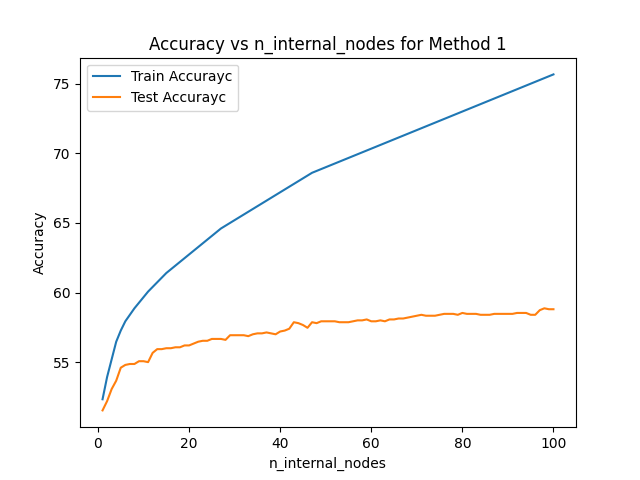
\includegraphics[width=0.5\textwidth]{Method1.png}

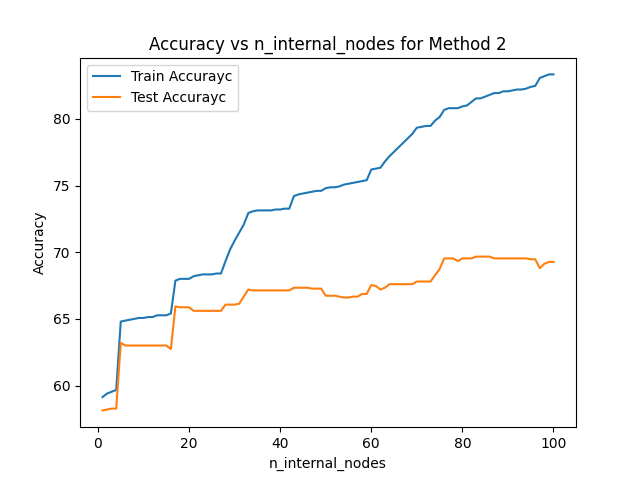
\includegraphics[width=0.5\textwidth]{Method2.png}

\section{2}

\subsection{a}

\begin{minted}{text}
       Trav        OC -> CRP
    /    |        /
  v      v       v 
FP  <- Fraud -> IP
\end{minted}

\begin{align*}
  P(OC) &= 0.6 \\
  P(!OC) &= 0.4 \\
  p(Trav) &= 0.05 \\
  P(!Trav) &= 0.95 \\
  P(Fraud | Trav) &= 0.01 \\
  P(!Fraud | Trav) &= 0.99 \\
  P(Fraud | !Trav) &= 0.004 \\
  P(!Fraud | !Trav) &= 0.996 \\
  P(FP | Trav + Fraud) = P(FP | Trav + !Fraud) &= 0.9 \\
  P(!FP | Trav + Fraud) = P(!FP | Trav + !Fraud) &= 0.1 \\
  P(FP | !Trav + Fraud) &= 0.1 \\
  P(!FP | !Trav + Fraud) &= 0.9 \\
  P(FP | !Trav + !Fraud) &= 0.01 \\
  P(!FP | !Trav + !Fraud) &= 0.99 \\
  P(IP | OC + Fraud) &= 0.02 \\
  P(!IP | OC + Fraud) &= 0.98 \\
  P(IP | OC + !Fraud) &= 0.01 \\
  P(!IP | OC + !Fraud) &= 0.99 \\
  P(IP | !OC + Fraud) &= 0.011 \\
  P(!IP | !OC + Fraud) &= 0.989 \\
  P(IP | !OC + !Fraud) &= 0.001 \\
  P(!IP | !OC + !Fraud) &= 0.999 \\
  P(CRP | OC) &= 0.1 \\
  P(!CRP | OC) &= 0.9 \\
  P(CRP | !OC) &= 0.001 \\
  P(!CRP | !OC) &= 0.999 \\
\end{align*}

\subsection{b}

\begin{align*}
  P(Fraud) &= \sum_{Trav, FP, IP, OC, CRP} P(Trav) P(OC) P(Fraud | Trav) P(FP | Trav + Fraud) \\ 
  &P(IP | OC + Fraud) P(CRP | OC) \\
  P(Fraud, FP) &= \sum_{Trav} P(Trav) P(Fraud | Trav) P(FP | Trav + Fraud) \\
  &= 0.05 \times 0.01 \times 0.9 + 0.95 \times 0.004 \times 0.1 = 0.00083\\
  P(Fraud, !FP) &= \sum_{Trav} P(Trav) P(Fraud | Trav) P(!FP | Trav + Fraud) \\
  &= 0.05 \times 0.01 \times 0.1 + 0.95 \times 0.004 \times 0.9 =0.00347\\
  P(Fraud) &= P(Fraud, FP) + P(Fraud, !FP) = 0.0043 \\
\end{align*}

\begin{align*}
  P(Fraud | FP + !IP + CRP) &= \sum_{Trav, OC} P(Trav) P(OC) P(Fraud | Trav) P(FP | Trav + Fraud) \\
  &P(IP | OC + Fraud) P(CRP | OC) \\
  F(Trav, OC) &= 0.05 \times 0.6 \times 0.01 \times 0.9 \times 0.02 \times 0.1 = 5.4e-7 \\
  F(Trav, !OC) &= 0.05 \times 0.4 \times 0.01 \times 0.9 \times 0.011 \times 0.001 = 1.98e-9 \\
  F(!Trav, OC) &= 0.95 \times 0.6 \times 0.004 \times 0.1 \times 0.02 \times 0.1 = 4.56e-7 \\
  F(!Trav, !OC) &= 0.95 \times 0.4 \times 0.004 \times 0.1 \times 0.011 \times 0.001 = 1.672e-9 \\
  P(Fraud | FP + !IP + CRP) &= \frac{F(Trav, OC) + F(Trav, !OC) + F(!Trav, OC) + F(!Trav, !OC)}{P(Fraud)} \\
  &= \frac{5.4e-7 + 1.98e-9 + 4.56e-7 + 1.672e-9}{0.0043} = 0.00023
\end{align*}

\subsection{c}

You want to make a computer purchase so that the system increases its probability of you owning a computer, which in turn reduces the probability of fraud.


\end{document}